\section{continous wavelet transformation}

The wavelet transform is used to see the frequency components of the signal in the time frequency domain. Wavelet transformation is practical when looking for signals of lower frequencies compared to the normal fourier analysis, because of the bigger resolution in the wavelet analysis. \cite{Greyer2004} Another drawback of the fourier transform is the loss of time information. 

The wavelet transformations is using a variable sized region windowing technique. Long time intervals are used where low frequency information is computed and short time intervals are used where high frequency information is computed. 

\begin{figure}[H]
	\centering	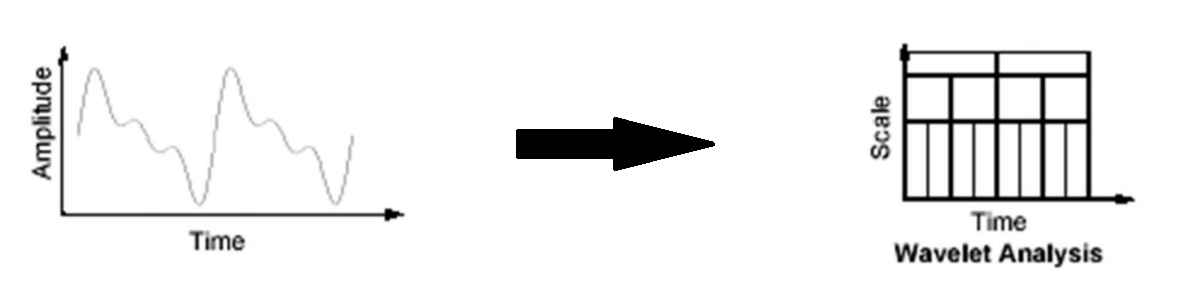
\includegraphics[width=0.65\textwidth]{figures/signalToWavelet}
	\caption{Signal to wavelet computation, modified from \cite{Uvo1995}}
	\label{fig:sigToWave}
\end{figure} \vspace{-.3cm}

The wavelet computes both the scale(s) and position(p) for the wavelet transform. 

\begin{flalign}
	C(s,p)=\int_{-\infty}^{\infty}f(t)\Psi (s,p) dt
	\label{eq:wave}
\end{flalign}

The signal f(t) is convoluted with the wavelet $\Psi$ to get the wavelet coefficients for s and p. 

This is done by computing the wavelet of the signal which then is compared to the wavelet for a section at the beginning of the signal. Then C in \ref{eq:wave} is calculated for the section of the signal. The wavelet is shifted to the right and repeated until the entire signal is covered. The wavelet is then scaled and C is computed for the entire signal again for all scales.

\begin{flalign}
W(t,s) \equiv \int_{-\infty}^{\infty} \frac{1}{s^n} \psi *(\frac{\tau-t}{\s})x(\tau)d\tau
\label{eq:cwt}
\end{flalign}

\begin{flalign}
	W(t,s) = \frac{1}{2\pi} \int_{-\infty}^{\infty} \Psi*(s\omega)X(\omega)e^{i\omega t} d\omega
	\label{eq:cwt2}
\end{flalign}

The signal which also is a function is put into the wavelet transformation \ref{eq:cwt}.